\section{Pandas}
Pandas is a data manipulation and analysis software library created for the Python programming language. It provides data structures and functions for manipulating numerical tables and time series. It is free software distributed under the BSD three-clause licence~\cite{Misc:OpenLDAP_license:oldap-2.7}.
The name derives from the words ``panel data'', which is an econometrics term for data sets that comprise observations for the same individuals over several time periods and, at the same time, is a parody of the term ``Python data analysis''~\cite{mckinney_data_2010}.

\subsection{Series and DataFrame}
Pandas is primarily used to analyse data. It supports data import from a variety of file formats, including comma-separated values (CSV), JSON, SQL database tables or queries, and Microsoft Excel~\cite{Misc:pandas_docs}.
Furthermore, Pandas supports a variety of data manipulation operations such as merging, reshaping, and selecting, as well as data cleaning and handling.
To accomplish these goals, Pandas defines and makes use of two important software \textit{Classes}, Series and DataFrame, which we will now briefly introduce.
\begin{figure}[ht]
    \centering
    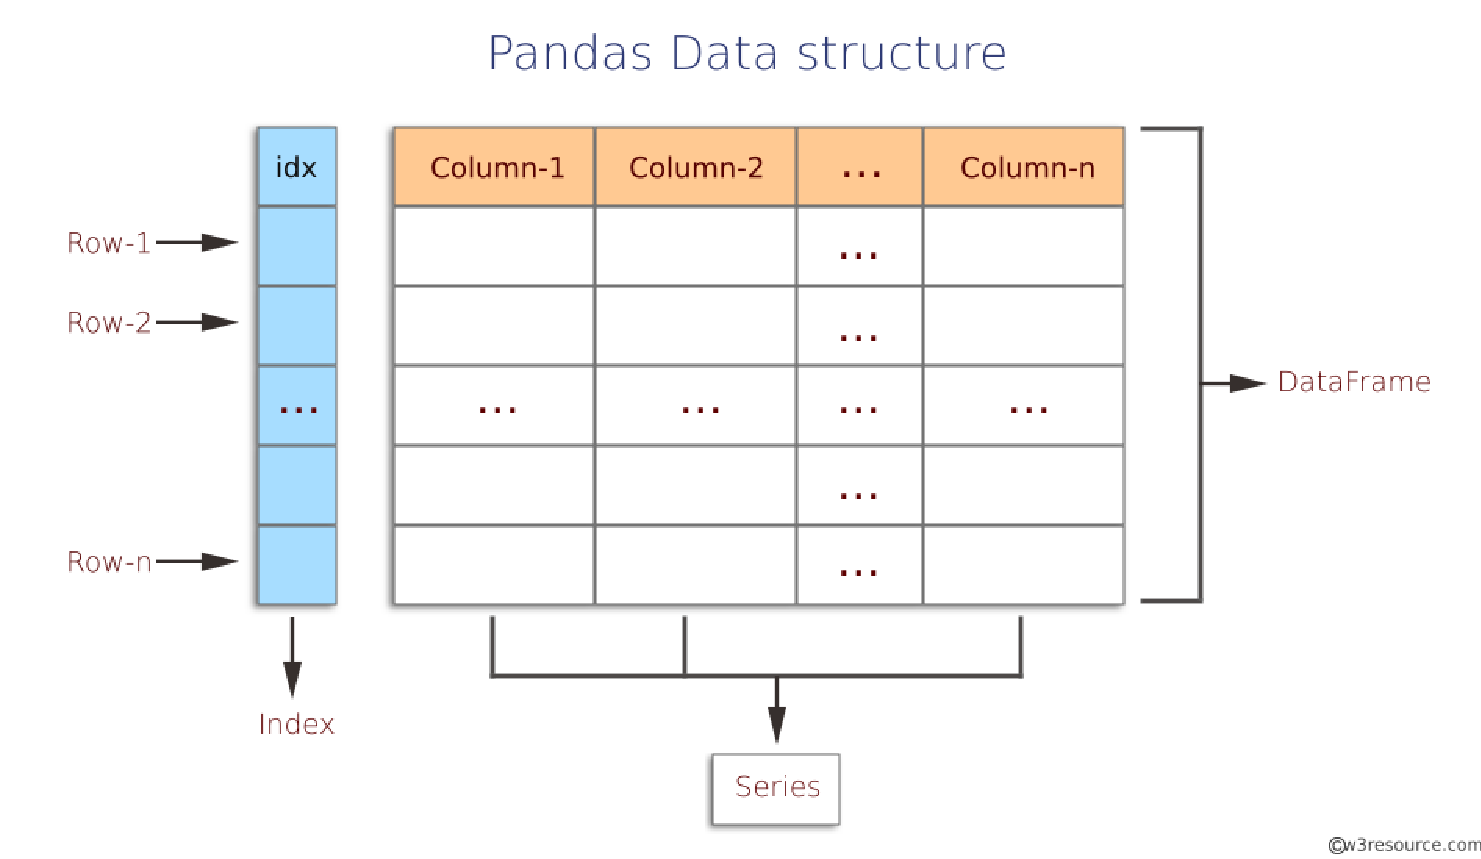
\includegraphics[width=\textwidth]{content/chapter_3/images/datastructure.pdf}
    \caption{Pandas Data structure}
    \label{fig:pandas_dataframe}
\end{figure}

\paragraph{Series} is a one-dimensional labeled array capable of holding any data type (integers, strings, floating point numbers, Python objects, etc.). 
The axis labels are collectively referred to as the \textit{index}.

\paragraph{DataFrame} is a 2-dimensional labeled data structure with columns of potentially different types; in some ways it is similar to
% EB: attenzione "it's like" e` informale
a spreadsheet or an SQL table (see Figure~\ref{fig:pandas_dataframe}) in which each individual column is a \textit{Series}.
It is, generally, the most commonly used pandas object, since it accepts many different kinds of input, which makes it very flexible~\cite{reback_pandas-dev/pandas:_2022}.
% \todo{EB: controllare Inglese next ``at makes him''?? Chi?? Se \`e Pandas ``it'' non ``him''}
Along with the data, user
% one 
can optionally pass index (row labels) and columns (column labels) arguments. By doing so, the user guarantees the index and/or columns of the resulting DataFrame.
% DG: ho riformulato specificando il soggetto:
% alternativamente to secure\ to ensure per \todo{EB: ``guaranteeing the index'' non suona bene}
If axis labels are not passed, they will be constructed from the input data based on common sense rules.
And this is just one way of building a Dataframe, an appetizer of the flexibility of this library.
% \todo{EB: non so se esista ``foretaste''. Io conosco ``appetizer'' in contesti simili, ma vedi tu}

\subsection{Core Features}
The goal
% idea
of this subsection is to give an outline of how many possible use-cases are covered by this library, and, at the same time, to explore a couple of them that proved to be crucial during my internship experience.
% \todo{EB: ``Let's start'' \`e troppo informale. Meglio qualcosa come ``We are now first  illustrate ...''}
We are now first illustrate the concept of "grouping". \textit{grouping}.

\paragraph{Groupby}
The name \textbf{GroupBy} should be quite familiar to those who have used a SQL-based tool or worked with relation database. This ``engine'' allows split-apply-combine operations on heterogeneous data sets.
By ``group by'' we are referring to a process involving one or more of the following steps:
\begin{enumerate}
    \item Splitting the data into groups based on some criteria.
    \item Applying a function to each group independently.
    \item Combining the results into a data structure
\end{enumerate}
\begin{figure}[ht]
    \centering
    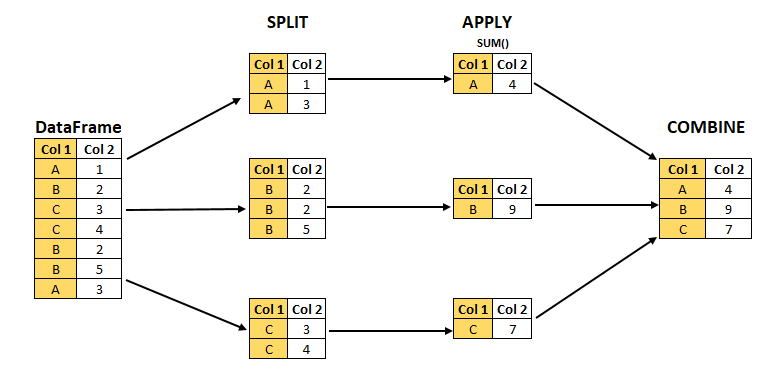
\includegraphics[width=\textwidth]{content/chapter_3/images/split-apply-combine.png}
    \caption{Shows the Split-Apply-Combine using an aggregation function (source: Analytics Vidhya~\cite{Misc:pandey_split-apply-combine})}\label{fig:pandas_groupby}
\end{figure}
Among these three steps, the \textit{split} is the most straightforward. In fact, in many situations, we would like to split the data set into groups and do something with those groups~\cite{reback_pandas-dev/pandas:_2022}.
In the \textit{apply and combine} step, we might wish to do one of the following:
\begin{itemize}
    \item Aggregation: compute a summary statistic (or statistics) for each group, some examples:
          \begin{itemize}
              \item Compute group sums or means.
              \item Compute group sizes / counts.
          \end{itemize}
    \item Transformation: perform some group-specific computations and return a like-indexed object, for instance:
          \begin{itemize}
              \item Standardize data (zscore) within a group.
              \item Filling NAs (value that are not valid) within groups with a value derived from each group.
          \end{itemize}
    \item Filtration: discard some groups, according to a group-wise computation that evaluates True or False, like:
          \begin{itemize}
              \item Discard data that belongs to groups with only a few members.
              \item Filter out data based on the group sum or mean.
          \end{itemize}
    \item Some combination of the above: \textbf{GroupBy} will examine the results of the \textit{apply} step and try to return a sensibly \textit{combined} result if it doesn't fit into either of the above two categories.
          \todo{EB: non capisco ``sensibly'' next, DG: ho scritto la traduzione, spero sia più chiaro, se no riformulo}
    \item Una qualche combinazione delle precedenti: GroupBy esaminerà i risultati del passo apply e cercherà di restituire un risultato sensatamente combinato se non rientra in nessuna delle due categorie precedenti.
\end{itemize}
Since the set of object instance methods on pandas data structures are generally rich and expressive, we often simply want to invoke, say, a DataFrame function on each group.
With this engine you can try multiple different approaches, testing what suits more your needs, even though often it is hard to define this three separate steps for badly shaped data.

\paragraph{Time series resampling}
Pandas contains extensive capabilities and features for working with time series data for all domains. Using the \textbf{NumPy} datetimes dtypes, it has consolidated a large number of features from other Python libraries (like \textbf{scikits.timeseries}) as well as created a tremendous amount of new functionality for manipulating time series data.
As an example, Pandas supports:
\begin{itemize}
    \item Parsing time series information from various sources and formats
    \item Manipulating and converting date times with timezone information
    \item Moving window statistics and linear regressions
\end{itemize}
\begin{figure}[ht]
    \centering
    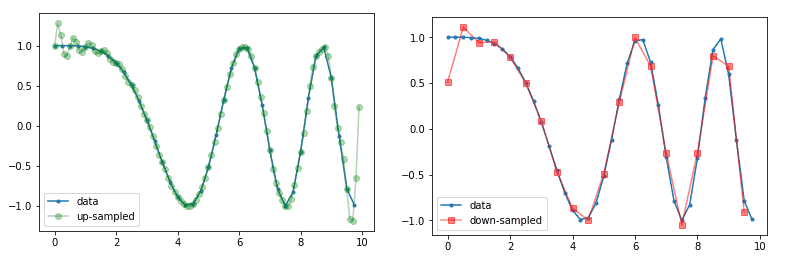
\includegraphics[width=\textwidth]{content/chapter_3/images/up-down-sample.png}
    \caption{Examples of signal waveform data processed by resample}\label{fig:up and down sampling}
\end{figure}
Let us now focus on one key aspect of handling/manipulating sensor data, crucial in our context, the necessity of resampling.
Fortunately, Pandas has, once again, a simple-to-use, powerful, and efficient functionality for performing resampling operations during frequency conversion
% \todo{EB: non sono sicuro dell'uso in Inglese di ``secondly'' e ``inutely''. Vedi un po' tu}
% l'ho preso dalla documentazione ufficiale https://pandas.pydata.org/docs/user_guide/timeseries.html#:~:text=(e.g.%2C%20converting%20secondly%20data%20into%205%2Dminutely%20data)
(e.g., converting secondly data into 5-minutely data). This is also extremely common in, but not limited to, financial applications~\cite{Misc:pandas_docs}.

To keep things simple, we could say that resample is a time-based \textbf{Groupby} followed by a reduction method on each of its groups; as a positive side,
this method can be used directly from \textit{DataFrameGroupBy} objects that we discussed in paragraph \textbf{GroupBy} previously discussed.
% \todo{EB: attenzione, i paragrafi non possono essere riferiti. Infatti, la label viene espansa con il numero della sezioine. Considerare se inserire ``il paragrafo XYZ in SectionXYZ''}
The resample function is very flexible and allows you to specify many different parameters to control the frequency conversion and resampling operation, both upsampling and downsampling.
%%%
\paragraph{Others functionality}
Furthermore, other time series features are available, and not only that notably:
\begin{itemize}
    \item Date range generation and frequency conversions
    \item Data alignment, shifting and lagging
    \item Integrated missing data handling
    \item Data set reshaping, pivoting, merging and combining
    \item Label-based slicing, sophisticated indexing, and big data set sub-setting
    \item Insertion and deletion of columns in a data structure.
\end{itemize}
\paragraph{Conlcusion}
Pandas provides a solid foundation upon which a very powerful data analysis ecosystem can be established, especially since the library is performance-optimized,
with important code paths implemented in Cython or C.
\todo{Cython \`e una roba moderna di voi giovani? Oppure \`e un typo?}
No è un compilatore statico e ottimistico per poter estendere Python con potenti librerie in C: https://cython.org/
``Cython gives you the combined power of Python and C''